\subsection{Sistema generado por el ACG}
	\label{sec:EJEMPLO1_ACG}
	
	En base a la red de grafos, ilustrada en la Figura \ref{fig:EJ1_8}, el ACG determinó la cantidad de elementos ferroviarios de cada tipo, tal como puede visualizarse en el Código \ref{lst:EJ1_8}.
	
	\begin{lstlisting}[language = {}, caption = Cantidad de elementos a implementar por el ACG, label = {lst:EJ1_8}]
	n_netElements:11
	n_switch:5
	n_doubleSwitch:0
	n_borders:4
	n_buffers:3
	n_levelCrossings:2
	n_platforms:2
	n_scissorCrossings:0
	n_signals:23
	N : 62
	\end{lstlisting}
	
	El ACG genera, en el caso de este ejemplo, 80 archivos en formato VHDL, tal como se puede visualizar en la Figura \ref{fig:EJ1_ACG_1}. Podemos destacar de la Figura \ref{fig:EJ1_ACG_1} al archivo \textit{Arty\_Z7-10.XDC}, que define los pines de entrada y salida de la plataforma Arty Z7 10 y Arty Z7 20. Este archivo es provisto por Xilinx para esta familia de plataformas. En caso de utilizar otra plataforma, se deberá incluir el archivo XDC correspondiente. En ambos casos, cada desarrollador debe asignar manualmente los pines a cada puerto del sistema generado por el ACG.
	
	\begin{figure}[H]
		\centering
		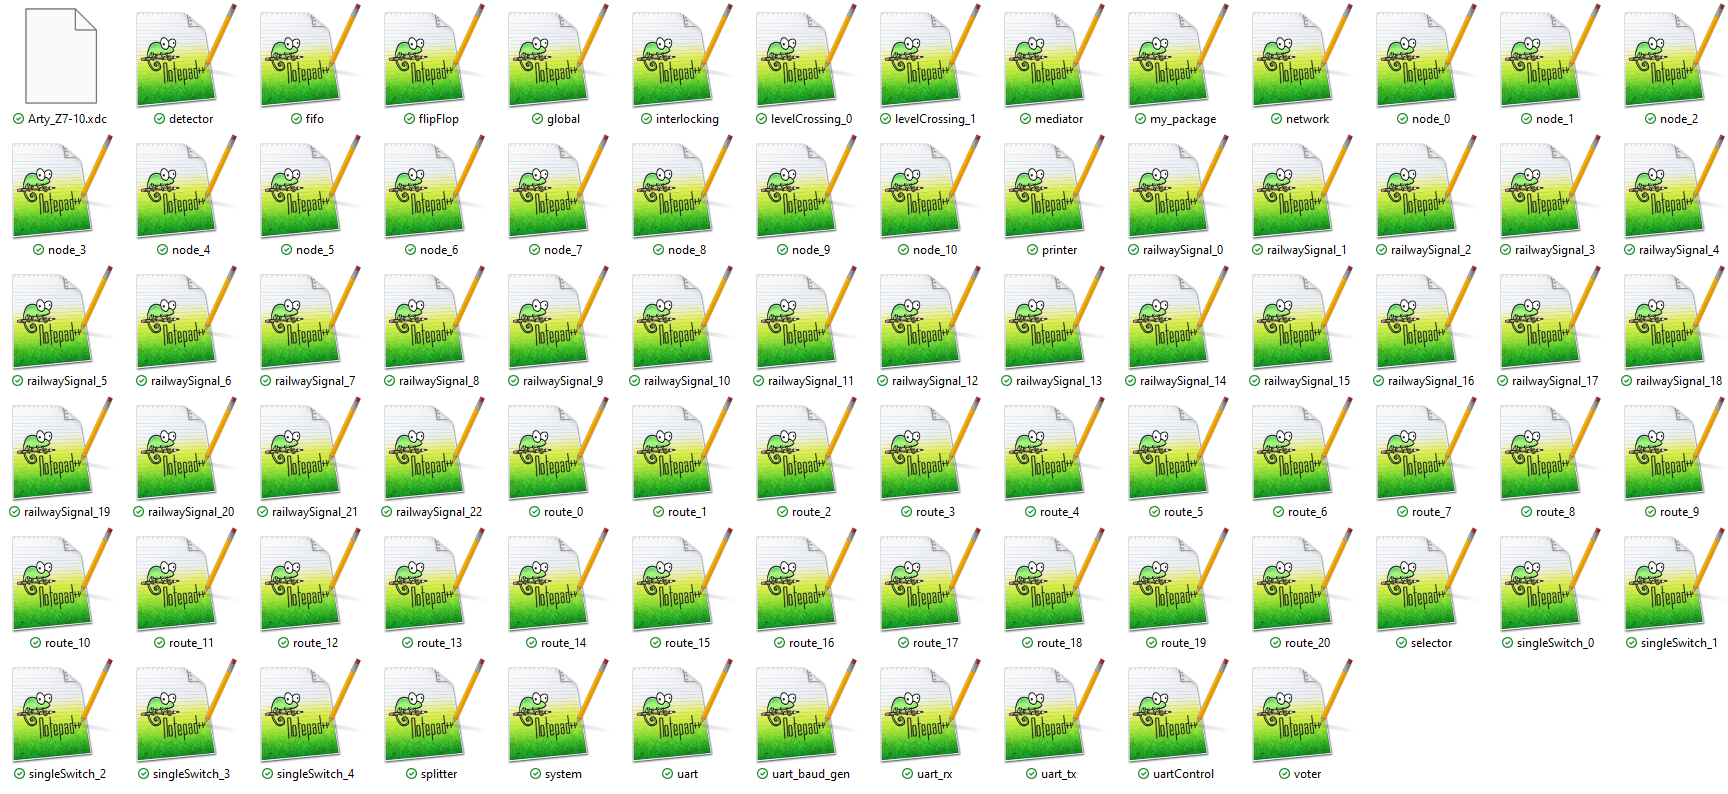
\includegraphics[origin = c, width=1\textwidth]{resultados-obtenidos/ejemplo1/images/ACG_files}
		\centering\caption{Archivos generador por el ACG para el ejemplo 1.}
		\label{fig:EJ1_ACG_1}
	\end{figure}
	
	Además, podemos mencionar los archivos \textit{my\_package.VHDL} y \textit{flipFlop.VHDL}, ambos generados por el ACG. El primero es una librería que define todos los tipos de datos utilizados por el sistema, y el segundo es un flip-flop tipo D utilizado para generar la secuencia de shift registers necesarios para adaptar el clock de entrada a los diferentes dominios de clock necesarios para el timeout de cada elemento ferroviario.
	
	Los archivos restantes son archivos que definen los módulos de alto nivel explicados en la Sección \ref{sec:interlockingArch} o la representación en VHDL de cada elemento ferroviario explicado entre la Sección \ref{sec:ACG_lc} y la Sección \ref{sec:ACG_rts}. Por ejemplo, en base lo descrito en el Código \ref{lst:EJ1_8}, hay 23 señales ferroviarias y podemos visualizar en la Figura \ref{fig:EJ1_ACG_1} 23 archivos referidos a las señales ferroviarias: desde \textit{railwaySignal\_0} hasta \textit{railwaySignal\_22}. Un ejemplo de la complejidad y profundidad del código generado es el archivo \textit{route\_13} que se puede visualizar en el Código \ref{lst:EJ1_vhdl}.	
	
	\begin{lstlisting}[language = {vhdl}, caption = route\_13.vdhl, label = {lst:EJ1_vhdl}, tabsize=2, basicstyle=\footnotesize\ttfamily]
--  route_13.vhdl : Automatically generated using ACG
	library IEEE;
	use IEEE.std_logic_1164.all;
	use IEEE.numeric_std.all;
	library work;
--Declare the package
	use work.my_package.all;
	entity route_13 is
	port(
		clock : in std_logic := '0';
		reset : in std_logic := '0';
		routeRequest : in hex_char;
		track_ne12 : in hex_char;
		ne12_command : out routeCommands := RELEASE;
		track_ne2 : in hex_char;
		ne2_command : out routeCommands := RELEASE;
		Sw06_state : in hex_char;
		Sw06_command : out routeCommands := RELEASE;
		C25_state : in hex_char;
		C25_command : out routeCommands := RELEASE;
		L08_state : in hex_char;
		L08_command : out routeCommands := RELEASE;
		routeExecute : out hex_char
	);
	end entity route_13;
	
	architecture Behavioral of route_13 is
		component flipFlop is
		port(
			clock : in std_logic := '0';
			reset : in std_logic := '0';
			Q : out std_logic := '0'
		);
		end component flipFlop;
	signal restart : std_logic := '1';
	signal Q : std_logic_vector(32 downto 0) := (others => '0');
	signal clock_in : std_logic_vector(32 downto 0) := (others => '0');
	signal timeout : std_logic := '0';
	signal routeState : routeStates := WAITING_COMMAND;
	signal routingIn : routeStates;
	signal ne12_used , ne2_used : std_logic := '0';
	signal ne12_state : nodeStates := FREE;
	signal ne12_lock : objectLock := RELEASED;
	signal ne2_state : nodeStates := FREE;
	signal ne2_lock : objectLock := RELEASED;
	signal Sw06_position : singleSwitchStates := NORMAL;
	signal Sw06_lock : objectLock := RELEASED;
	signal C25_aspectIn : signalStates := RED;
	signal C25_lock: objectLock := RELEASED;
	signal L08_aspectIn : signalStates := RED;
	signal L08_lock : objectLock := RELEASED;
	begin
		clock_in(0) <= clock;
		routingIn <= routeStates'val(to_integer(unsigned(hex_to_slv(routeRequest))));
		routeExecute <= slv_to_hex(std_logic_vector(to_unsigned(routeStates'pos(routeState),4)));
		ne12_state <= nodeStates'val(to_integer(unsigned(hex_to_slv(track_ne12)(2 to 3))));
		ne12_lock <= objectLock'val(to_integer(unsigned(hex_to_slv(track_ne12)(0 to 1))));
		ne2_state <= nodeStates'val(to_integer(unsigned(hex_to_slv(track_ne2)(2 to 3))));
		ne2_lock <= objectLock'val(to_integer(unsigned(hex_to_slv(track_ne2)(0 to 1))));
		Sw06_position <= singleSwitchStates'val(to_integer(unsigned(hex_to_slv(Sw06_state)(2 to 3))));
		Sw06_lock <= objectLock'val(to_integer(unsigned(hex_to_slv(Sw06_state)(0 to 1))));
		C25_aspectIn <= signalStates'val(to_integer(unsigned(hex_to_slv(C25_state)(2 to 3))));
		C25_lock <= objectLock'val(to_integer(unsigned(hex_to_slv(C25_state)(0 to 1))));
		L08_aspectIn <= signalStates'val(to_integer(unsigned(hex_to_slv(L08_state)(2 to 3))));
		L08_lock <= objectLock'val(to_integer(unsigned(hex_to_slv(L08_state)(0 to 1))));
	
		gen : for i in 0 to 31 generate
			inst: flipFlop port map(clock_in(i), restart, Q(i));
			clock_in(i+1) <= Q(i);
		end generate;
	
		process(clock,reset,Q,restart)
		begin
			if (reset = '1' or Q = "011011111100001000111010101111110") then
				timeout <= '1';
			end if;
			if (restart = '1') then
				timeout <= '0';
			end if;
		end process;
		
		process(clock)
		begin
			if (clock'Event and clock = '1') then
				case routeState is
					when WAITING_COMMAND =>
					if (routingIn = ROUTE_REQUEST) then
						routeState <= RESERVING_TRACKS;
					end if;
					when RESERVING_TRACKS =>
						restart <= '0';
						if (routingIn = CANCEL_ROUTE or timeout ='1') then
							routeState <= CANCEL_ROUTE;
						end if;
						if ((ne12_lock = RELEASED and ne2_lock = RELEASED) and (ne2_state = FREE)) then
							ne12_command <= RESERVE;
							ne2_command <= RESERVE;
						end if;
						if (ne12_lock = RESERVED and ne2_lock = RESERVED)then
							restart <= '1';
							routeState <= LOCKING_TRACKS;
						end if;
			when LOCKING_TRACKS =>
				restart <= '0';
				if (routingIn = CANCEL_ROUTE or timeout ='1') then
					routeState <= CANCEL_ROUTE;
				end if;
				if ((ne12_lock = RESERVED and ne2_lock = RESERVED) and (ne2_state = FREE)) then
					ne12_command <= LOCK;
					ne2_command <= LOCK;
				end if;
				if (ne12_lock = LOCKED and ne2_lock = LOCKED)then
					restart <= '1';
					routeState <= RESERVING_INFRASTRUCTURE;
				end if;
			when RESERVING_INFRASTRUCTURE =>
				restart <= '0';
				if (routingIn = CANCEL_ROUTE or timeout ='1') then
					routeState <= CANCEL_ROUTE;
				end if;
				if (Sw06_lock = RELEASED) then
					Sw06_command <= RESERVE;
				end if;
				if (Sw06_lock = RESERVED)then
					restart <= '1';
					routeState <= LOCKING_INFRASTRUCTURE;
				end if;
			when LOCKING_INFRASTRUCTURE =>
				restart <= '0';
				if (routingIn = CANCEL_ROUTE or timeout ='1') then
					routeState <= CANCEL_ROUTE;
				end if;
				if (Sw06_lock = RESERVED) then
					Sw06_command <= LOCK;
				end if;
				if (Sw06_lock = LOCKED)then
					ne12_used <= '0';
					ne2_used <= '0';
					restart <= '1';
					routeState <= DRIVING_SIGNAL;
				end if;
			when DRIVING_SIGNAL =>
				restart <= '0';
				if (routingIn = CANCEL_ROUTE or timeout ='1') then
					routeState <= CANCEL_ROUTE;
				end if;
				if (C25_lock = RELEASED and L08_lock = RELEASED) then
					C25_command <= RESERVE;
					L08_command <= LOCK;
				end if;
				if (C25_lock = RESERVED and L08_lock = LOCKED) then
					restart <= '1';
					routeState <= SEQUENTIAL_RELEASE;
				end if;
			when SEQUENTIAL_RELEASE =>
				restart <= '0';
				if (routingIn = CANCEL_ROUTE or timeout ='1') then
					routeState <= CANCEL_ROUTE;
				end if;
				--- Sequential release
				if (ne12_used = '0' and ne12_state = OCCUPIED) then 
					ne12_used <= '1';
				end if;
				if (ne12_used = '1' and ne12_state = FREE) then
					ne12_used <= '0';
					ne12_command <= RELEASE;
				end if;
				---
				if (ne12_lock = RELEASED and ne2_used = '0' and ne2_state = OCCUPIED) then 
					ne2_used <= '1';
					--- Finish -> Release all
					restart <= '1';
					routeState <= RELEASING_INFRASTRUCTURE;
				end if;
			when RELEASING_INFRASTRUCTURE =>
				Sw06_command <= RELEASE;
				ne12_command <= RELEASE;
				ne2_command <= RELEASE;
				C25_command <= RELEASE;
				L08_command <= RELEASE;
				restart <= '1';
				routeState <= WAITING_COMMAND;
			when CANCEL_ROUTE =>
				routeState <= RELEASING_INFRASTRUCTURE;
			when others =>
				routeState <= WAITING_COMMAND;
			end case;
		end if;
		end process;
	end Behavioral;
	\end{lstlisting}
	
	El Código \ref{lst:EJ1_vhdl} incluye la declaración de puertos, la creación de las variables necesarias, la conversión de tipos de datos, la conexión de flip-flops para generar un shift-register tal que se puedan utilizar como timeout con las condiciones prefijadas y la máquina de estados de la ruta, tal como se explicó en la Sección \ref{sec:ACG_rts}.
	
	Cada ejemplo cuenta con su propia carpeta de principio a fin. Es decir, el archivo railML original, los archivos generados por el RNA y el código generado por el ACG se encuentran en carpetas individuales para cada ejemplo. Esto es una ventaja a la hora de mantener un orden pero una gran desventaja a la hora de sintetizar los proyectos en Vivado. Cada conjunto de archivos debería ser importado de manera individual, previa desvinculación de los archivos del proyecto anterior. Para solucionar este inconveniente se desarrolló el Código \ref{lst:EJ1_script}, que automatiza la importación y desvinculación de los archivos de cada ejemplo.
	
	\begin{lstlisting}[language = {bash}, caption = script.tcl, label = {lst:EJ1_script}]
set chosen 1

# Get a list of all design source files
set design_sources [get_files -of_objects [get_filesets sources_1]]

remove_files $design_sources

set base_folder_path "ROOT/GICSAFePhD/App/Layouts/Example_"
set folder_path "${base_folder_path}${chosen}/VHDL"

puts $folder_path

set files [glob -directory $folder_path *.vhd]

add_files -norecurse -scan_for_includes  $files

update_compile_order -fileset sources_1
update_compile_order -fileset sources_1

synth_design -rtl -rtl_skip_mlo -name rtl_1
	\end{lstlisting}
	
	El parámetro \textit{chosen} indica el número de ejemplo seleccionado, mientras que \textit{base\_folder\_path} es la ruta absoluta de los ejemplos, cuyas carpetas deben ser nombradas como \textit{Example\_}+\textit{chosen} para poder ser encontradas. El Código \ref{lst:EJ1_script} puede ser importado en Vivado desde \textit{Tools $>$ Custom Commands $>$ Customize Commands} como un archivo TCL (del inglés, Tool Command Language), que es el formato que define los comandos nativos de Vivado. Pueden importarse tantos archivos TCL como se deseen, uno por cada ejemplo a sintetizar. De esta manera, cada script aparecerá en la barra de acceso rápido de Vivado de forma independiente y se automatiza el proceso de sincronización de archivos.
	
	Una vez ejecutado el script, Vivado ordenará los archivos de forma jerárquica, como puede verse en la parte izquierda de la Figura \ref{fig:EJ1_ACG_Vivado} donde el módulo \textit{global} incluye todos los módulos que fueron detallados en la Sección \ref{sec:interlockingArch}. Podemos destacar al módulo \textit{network} que es instanciado 3 veces junto con el módulo \textit{voter}, al ser una redundancia 2oo3, tal fue explicado en la Sección \ref{sec:VHDL2oo3}. Cada una de las instancias del módulo \textit{network} contienen sus propias 62 instancias de los mismos módulos de cada elemento ferroviario ya que N, cantidad de elementos ferroviarios, es 62 en el Código \ref{lst:EJ1_8}.	
	
	\begin{figure}[H]
		\centering
		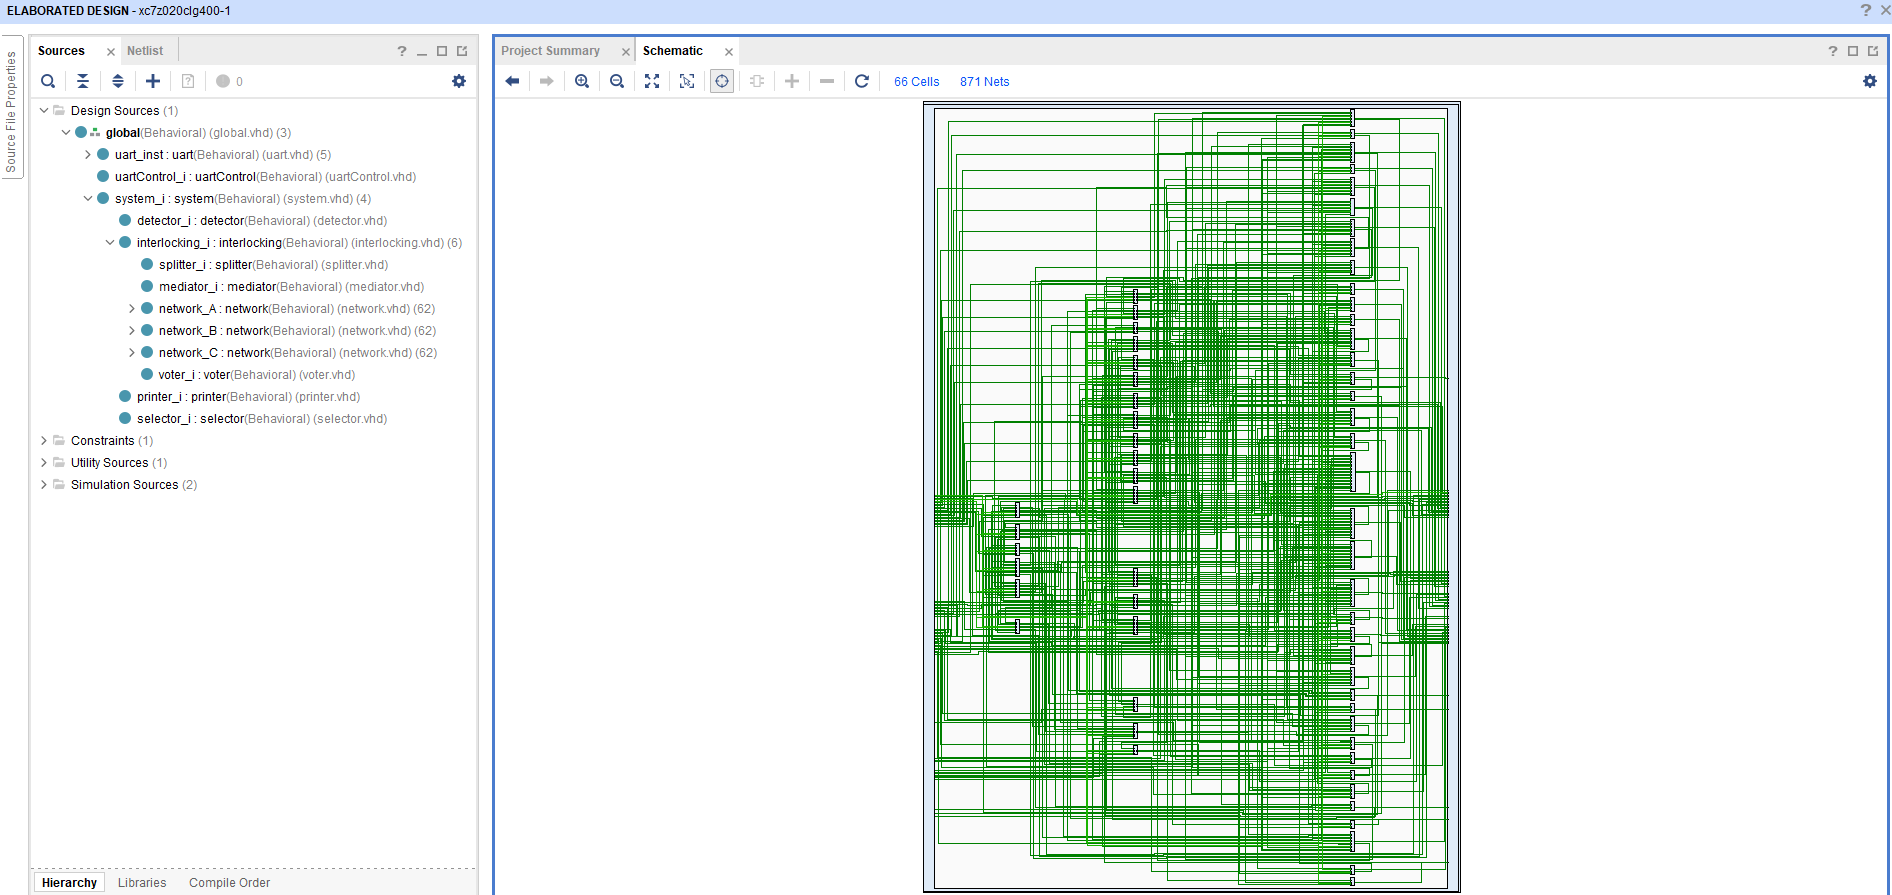
\includegraphics[origin = c, width=1\textwidth]{resultados-obtenidos/ejemplo1/images/ACG_vivado}
		\centering\caption{Interfaz del entorno de desarrollo Vivado para el ejemplo 1.}
		\label{fig:EJ1_ACG_Vivado}
	\end{figure}
	
	La parte derecha de la Figura \ref{fig:EJ1_ACG_Vivado} ilustra la representación en diagrama de bloques de uno de los módulos \textit{network} (los tres módulos tienen los mismos bloques). Puede apreciarse en esta ventana que existen 66 módulos interconectados de forma compleja utilizando 871 señales. Pero esto es solamente una porción del sistema generado por el ACG, de inspeccionar cada uno de los bloques es posible determinar que el ejemplo 1 utiliza 9517 sub módulos conectados automáticamente mediante 21899 señales, lo cual se aleja bastante de un desarrollo que pueda realizarse manualmente de forma trivial.
	
	Una vez que Vivado ha generado el diagrama de bloques ya tenemos la certeza de que el código VHDL ha pasado la prueba de sintaxis del entorno de desarrollo. A continuación, se deberá sintetizar e implementar el sistema para generar el bitstream que será utilizado para programar la FPGA. Durante el proceso de síntesis, Vivado busca la mejor forma de representar el código VHDL con compuertas lógicas, por lo que un código de mejor calidad brindará una representación en hardware lo mas fiel posible a lo buscado. Durante el proceso de implementación, en cambio, Vivado calcula si la representación con compuertas lógicas es posible de realizarse con la plataforma disponible. En este proceso influye no solamente la cantidad de compuertas disponibles sino también el tipo de compuertas. Si la plataforma no cuenta con la cantidad suficiente de compuertas A, entonces Vivado buscará la forma de reemplazar esa compuerta por otras compuertas B, C o D, que sean su equivalente lógico. Este proceso de reemplazo y/o simplificación puede llevar a que ambos procesos presenten discrepancias en la cantidad de elementos utilizados. 
	
	Los resultados de ambos procesos son detallados en la Tabla \ref{Tab:tabla_ACG_1}. Los porcentajes de uso son calculados por Vivado automáticamente, teniendo en cuenta que la plataforma Arty Z7 20 posee 53200 Look-Up-Tables (LUTs), 106400 Flip-Flops (FFs), 125 Pines de entrada y salida (IOs) y 32 Buffers (BUFGs), tal cómo se explicó en la Sección \ref{sec:AGG}. En este ejemplo, la cantidad de recursos utilizados es baja y el tiempo de síntesis e implementación es de 47 y 44 segundos, respectivamente.
	
	\begin{table}[H]
		{
			\caption{Síntesis e implementación del ejemplo 1 generado por el ACG.}
			\label{Tab:tabla_ACG_1}
			\centering
			%\small
			%\centering
			\begin{center}
				\resizebox{0.7\textwidth}{!}{
					\begin{tabular}{ c c c c }
						\hline	
						Recursos & Síntesis & Implementación & Uso \\	
						\hline
						LUT & 3457 & 3416 & 6.42/6.50\%\\
						FF & 3810 & 3813 & 3.58\%\\
						IO & 15 & 15 & 12.00\%\\
						BUFG & 3 & 3 & 9.38\%\\
						\hline
					\end{tabular}
				}
			\end{center}
		}    
	\end{table}
	
	
	